%!TEX root = ../aamas11storage.tex
% %%%%%%%%%%%%%%%%%%%%%%%%%%%%%%%%%%%%%%%%%%%%%%%%%%%
\section{A Dynamic Confidence Measure}\label{sec:confidence}
% %%%%%%%%%%%%%%%%%%%%%%%%%%%%%%%%%%%%%%%%%%%%%%%%%%%

In this section we describe a dynamic confidence measure that may be used to guide exploration when learning plan selection using the framework described in Section \ref{sec:framework}. Conceptually, the value of the confidence measure relates to the degree of trust that the agent has in its current understanding of the world (from a learning perspective). Technically, recall that the confidence metric informs the agent about how much it should trust the outcome estimate provided by its current decision tree.

Our new confidence measure improves upon previously used measures in two important ways. 
%
Firstly, it caters to changing dynamics of the environment that often results in prior learning becoming less effective. The stability-based \cite{airiau09:enhancing} and coverage-based \cite{singh10:extending,singh10:learning} measures that have been previously proposed do not support the requirement for adaptability to such changes. Moreover, the new measure proposed here subsumes the functionality of the former methods, as it behaves monotonically in environments where the dynamics are fixed. As such, it offers a direct replacement for the previous approaches. 
%
Secondly, the new measure does not rely on estimates of the number of choices in the goal-plan hierarchy as is the case in \cite{singh10:extending,singh10:learning}, and scales to any general goal-plan hierarchy irrespective of its complexity.


To recap the definition of stability from \cite{singh10:learning}:

\begin{quote}
\emph{``A failed plan $P$ is considered to be stable for a particular world state $w$ if the rate of success of $P$ in $w$ is changing below a certain threshold.''}
\end{quote} 

\newcommand{\ds}{\zeta}
\newcommand{\app}{\mathname{app}}
\newcommand{\stable}{\mathname{stable}}

Our aim is to use this notion to judge how ``stable'' or well-informed the decisions the agent has made within a particular execution trace were. This is particularly meaningful for \emph{failed} execution traces: low stability suggests that we were not well-informed and more exploration is needed before assuming that no solution is possible (for the trace's top goal in question).
%%
To capture this, we define the \emph{degree of stability} of a (failed) execution trace $\lambda$, denoted $\ds(\lambda)$ as the ratio of stable plans to total applicable plans in the active execution trace below the top-level goal event in $\lambda$. Formally, when $\lambda= G_1[P_1:w_1] \cdots G_n[P_n:w_n]$ we define 
%%
\[
\ds(\lambda) = 
	\frac{ 
			\card{ \bigcup_{i=1}^n \set{P \mid P \in \Delta_{\app}(G_i,w_i),\, \stable(P,w_i)} } 
		}
		{
			\card{	\bigcup_{i=1}^n \Delta_{\app}(G_i,w_i) } 
		},
\]

\noindent
where  $\Delta_{\app}(G_i,w_i)$ denotes the set of all applicable plans (i.e., whose boolean context conditions hold true) in world state $w_i$ for goal event $G_i$, and $\stable(P,w_i)$ holds true if plan $P$ is deemed stable at world state $w_i$, as defined in~\cite{singh10:learning}.

For instance, take the failed execution trace $\lambda = G[P:w] \cdot G_2[P_f:w_2] \cdot G_5[P_n:w_5]$ from before and suppose further that the applicable plans are $\Delta_{\app}(G,w) = \{P\}$, $\Delta_{\app}(G_2,w_2) = \{P_d,P_f\}$, and $\Delta_{\app}(G_5,w_5) = \{P_m,P_n,P_o\}$. Further assume that $P_d$ and $P_n$ are the only plans deemed stable (in worlds $w_2$ and $w_5$ respectively). 
%%
Then the degree of stability for the whole trace is $\ds(\lambda)= 2/6$.
%%
Similarly, for the two subtraces $\lambda'= G_2[P_f:w_2] \cdot G_5[P_n:w_5]$ and $\lambda'' =G_5[P_n:w_5]$ of $\lambda$, we get $\ds(\lambda') = 2/5$ and $\ds(\lambda'') = 1/3$.



\newcommand{\StablePlan}{\mathname{StablePlan}}
\newcommand{\SetDegreeStability}{\mathname{RecordDegreeStability}}
\newcommand{\UpdateDegreeStability}{\mathname{RecordDegreeStabilityInTrace}}

The idea is that every time the agent reaches a failed execution trace, the stability degree of each subtrace is stored in the plan that produced that subtrace.
%%
So, for our example, for plan $P$ we store degree $\ds(\lambda')$ whereas for plan $P_f$ we record degree $\ds(\lambda'')$. Leaf plan nodes, like $P_n$, make no choices so their degree is simply $1$.
%%
Intuitively, by doing this, we record against each plan in the (failed) trace, an estimate of how informed the current (active) choices made for the plan were.  
%%
Algorithm~\ref{alg:degree} describes how this (hierarchical) recording happens given an active execution trace $\lambda$. Observe how the stability measure is recorded against each plan in the trace: $\SetDegreeStability(P, w, d)$ records degree $d$ for plan $P$ in world state $w$.

\begin{algorithm}[h]
\KwData{$\lambda=G_1[P_1:w_1] \cdot \ldots \cdot G_n[P_n:w_n]$, with $n \geq 1$.}
% ; $s\geq0$; $t\geq0$; $k\geq0$; $\epsilon\geq0$}
\KwResult{Records degree of stability for plans in $\lambda$.}
\If{$(n > 1)$}{
% 	$t = \Sigma_{i \in \{1,\ldots,n\}} \card{\Delta_{\app}(G_i,w_i)}$\;
% 	$s = \Sigma_{i \in \{1,\ldots,n\}} \card{\Delta_{\app}(G_i,w_i)}$\;
	$\lambda'=G_2[P_2:w_2] \cdot \ldots \cdot G_n[P_n:w_n]$\;
	$d = \ds(\lambda')$\;  
	$\SetDegreeStability(P_1, w_1, d)$\;
% 	\ForEach{$P_i$ in $T_n$; $P_i \neq P_n$}{
% 		$s' = s' + \StablePlan(P_i, w_n, k,\epsilon)$\;
% 		$t' = t + 1$\;
% 	}
	$\UpdateDegreeStability(\lambda')$\;
}
\Else{$\SetDegreeStability(P_1, w_1, 1)$\;}
\caption{$\UpdateDegreeStability(\lambda)$}
\label{alg:degree}
\end{algorithm}


As a plan execution produces new failed experiences, the calculated degree of stability is appended against it each time. When a plan finally succeeds, we take an optimistic view and record $1$ (i.e., full stability) against it. This, together with the fact that all plans do eventually become stable, means that $\ds(\lambda)$ is guaranteed to converge to $1$. 


To aggregate the different stability recordings for a plan over time, we use the \emph{average degree of stability} over the last $n \geq 1$ executions of plan $P$ in $w$, denoted $\C_s(P,w,n)$. 
%%
This provides us with a measure of confidence in the decision tree for plan $P$ in state $w$. Intuitively, $\C_s(P,w,n)$ tells us how ``informed" the decisions taken when performing $P$ in $w$ were over the $n$ most recent executions.
%%
Notice that if the environment dynamics are constant, this measure monotonically increases from $0$, as plans below $P$ start to become stable (or succeed); it reaches $1$ when all tried plans below $P$ in the last $n$ executions are considered stable. This is what one might expect in the typical learning setting. However, if the environment dynamics were to change and plans start to fail or become unstable, then the measure behaves non-monotonically and adjusts confidence accordingly.


% \newcommand{\aSet}{\mathname{set}}
% \newcommand{\aOperate}{\mathname{operate}}
% \newcommand{\aEvaluate}{\mathname{evaluate}}
% 
% \newcommand{\pSet}{\mathname{Set*}}
% \newcommand{\pSetCharge}{\mathname{SetCharge}}
% \newcommand{\pSetDischarge}{\mathname{SetDischarge}}
% \newcommand{\pSetNotUsed}{\mathname{SetNotUsed}}
% \newcommand{\pExecute}{\mathname{Execute}}
% 
% \newcommand{\cSatisfies}{\psi}
% 
% \begin{figure*}[t]
% \begin{center}
% \subfigure[Use case scenario for a modular battery system.]{\label{fig:usecase}
% %\resizebox{0.9\columnwidth}{!}{
% %!TEX root = ../aamas11storage.tex
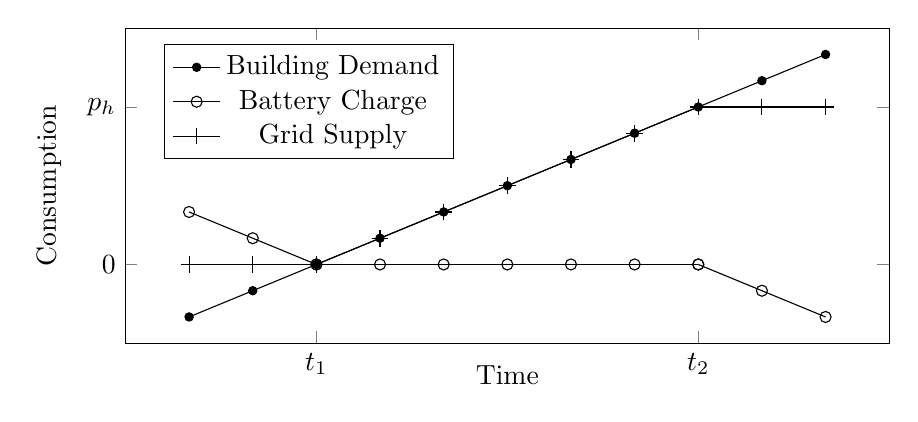
\begin{tikzpicture}

\begin{axis}[
width=0.8\columnwidth,height=4cm,scale only axis,
axis line style={-}, xtick style={-}, ytick style={-},
xlabel=Time,
ylabel=Consumption,
every axis y label/.style={at={(-0.1,0.5)},rotate=90,anchor=center}, 
every axis x label/.style={at={(0.5,-0.1)},anchor=center}, 
%grid=both, grid style={style=densely dotted},
xtick={2,8},
xticklabels={$t_1$,$t_2$},
ytick={0,6},
yticklabels={$0$,$p_h$},
legend style={at={(0.05,0.95)},anchor=north west}
] 

% Draw the Demand-Supply curve
\addplot[-,mark=*,mark size=1.5] expression[domain=0:10,samples=11] {x-2};
\addlegendentry{Building Demand} 

% Draw the Battery curve
\addplot[-,mark=o,mark size=2] expression[forget plot,domain=0:2,samples=3] {2-x}; 
\addplot[-,mark=o,mark size=2] expression[forget plot,domain=2:8,samples=7] {0}; 
\addplot[-,mark=o,mark size=2] expression[domain=8:10,samples=3] {8-x}; 
\addlegendentry{Battery Charge} 

% Draw the Grid supply curve
\addplot[-,mark=+,mark size=3] expression[forget plot,domain=0:2,samples=3] {0}; 
\addplot[-,mark=+,mark size=3] expression[forget plot,domain=2:8,samples=7] {x-2}; 
\addplot[-,mark=+,mark size=3] expression[domain=8:10,samples=3] {6}; 
\addlegendentry{Grid Supply} 
\end{axis} 
\end{tikzpicture} 

% %}
% }
% \qquad
% \subfigure[Goal-plan hierarchy for a $k$-modules battery system.]{\label{fig:gptree}
% %\resizebox{0.9\columnwidth}{!}{
% %!TEX root = ../aamas11storage.tex
\begin{tikzpicture} [level distance=8.0em]
\tikzstyle{planbox}=[draw,text width=11.0em,rectangle split,rectangle split parts=3]
\tikzstyle{goalbox}=[draw,rounded corners=1.25em,minimum height=3em,minimum width=5em]

	
\tikzstyle{level 1}=[sibling distance=13.0em] 
\tikzstyle{level 2}=[level distance=7.0em] 

\node[goalbox,solid] {$G($r,k,s$)$}
	child {node[planbox] {$SetCharge$ 
			\nodepart{second} $\psi:satisfies(r,k,s,C),$\\$k>0$
			\nodepart{third} $set(k,C)$
		}
		child {node[goalbox] {$G($r,k-1,s'$)$}}
	}
	child {node[planbox] {$SetDischarge$ \nodepart{second}
			\nodepart{second} $\psi:satisfies(r,k,s,D),$\\$k>0$
			\nodepart{third} $set(k,D)$
		}
		child {node[goalbox] {$G($r,k-1,s'$)$}}
	}
	child {node[planbox] {$SetNotUsed$ \nodepart{second}
			\nodepart{second} $\psi:satisfies(r,k,s,N),$\\$k>0$
			\nodepart{third} $set(k,N)$
		}
		child {node[goalbox] {$G($r,k-1,s'$)$}}
	}
	child {node[planbox] {$Execute$ 
			\nodepart{second} $\psi:k==0$
			\nodepart{third} $operate()$ \\$evaluate()$
		}
	}
;

\end{tikzpicture}



% %}
% }
% \caption{An energy storage application.}
% \end{center}
% \label{fig:energystorage}
% \end{figure*}


The stability-based confidence measure $\C_s(\cdot,\cdot,\cdot)$ would make a useful heuristic for exploration (i.e., plan selection) in its own right: when the confidence is at its lowest the agent does maximum exploration, and when it is at its highest, the agent fully utilises the decision trees. 
%%
A problem with this approach, though, is that such measure only covers the space of \emph{known} worlds. This means that whenever a new world is witnessed, this stability-based confidence will be zero, meaning that the agent will choose randomly. This is hardly beneficial since what we would really like is to use the learnt generalisations to classify (i.e. predict the outcome in) this new world rather than being agnostic about it. 
%%
What is missing is a complementary metric that contributes to our net confidence but that is independent of $w$.


\newcommand{\neww}{\mathname{NewStates}}
One way to address this limitation is by monitoring the rate at which new worlds are being witnessed by a  plan $P$. During early exploration, it is expected that the majority of worlds that a plan is selected for will be unique, thus yielding a high rate and a low confidence. Over time, as exploration continues, the plan would get selected in all worlds in which it is reachable and the rate of new worlds would approach zero, while our confidence over this period increases to its maximum.  
%%
So, we define our second confidence metric $\C_d(P,n) = |\neww(P,n)|/n$, where $\neww(P,n)$ is the set of world states that have been seen for the first time in the last $n$ executions of $P$.
%%
Clearly, $\C_d$ is guaranteed to converge to $1$ as long as all worlds where the plan might apply are eventually witnessed.

In summary, we have defined two confidence metrics over two orthogonal dimensions. Stability-based confidence $\C_s(P,w,n)$ is meant to capture how well-informed the last $n$ executions of plan $P$ in world $w$ were, whereas world-based confidence $\C_d(P,n)$ is meant to capture how well-known the worlds in the last $n$ executions of plan $P$ were, compared with what we had experienced before.


We now have all the technical machinery to define our final (aggregated) confidence measure $\C$ that takes into account both the above metrics. Specifically, the overall confidence in the decision tree of plan $P$ in world $w$ relative to the last $n$ experiences is defined as follows:
%%
\[
	\C(P,w,n) = \alpha\C_s(P,w,n) + (1-\alpha)\C_d(P,n),
\label{eqn:confidence}
\]

\noindent
where $\alpha$ is a weighting factor used to set a preference bias between the two component metrics.



Finally, we show how this confidence measure is to be used within the plan selection mechanism of a BDI agent. Remember that for a given goal-event that needs to be resolved, a BDI agent may have several applicable plans from which one ought to be selected for execution. The BDI learning framework described in Section~\ref{sec:framework} will chose probabilistically among these options in a way proportional to some given weight per plan---the more weight a plan is assigned, the higher the chances of it being chosen. 
%%
Following~\cite{singh10:extending, singh10:learning}, we define this selection weight for plan $P$ in world $w$ relative its last $n$ executions as follows: 
%%
\[
	\Omega(P,w,n) = 0.5 + \left[  \C(P,w,n) \times  \left( \P(P,w) - 0.5 \right)  \right],
\label{eqn:omega}   
\]

\noindent 
where $\P(P,w)$ is the probability of success of plan $P$ in world $w$ as given by $P$'s decision tree. 
%
Indeed, this weight definition is basically that of~\cite{singh10:extending, singh10:learning}, except for the use of our new confidence metric $\C(\cdot,\cdot,\cdot)$ as defined above. The idea is to combine the likelihood of success of plan $P$ in world $w$ (i.e. the term $\P(P,w)$) with a confidence bias (in this case $\C(\cdot,\cdot,\cdot) \in [0.0:1.0]$) to determine a final plan selection weight $\Omega(\cdot,\cdot,\cdot)$. 
%When the confidence is maximum, then $\Omega(\cdot,\cdot,\cdot) = \P(\cdot,\cdot)$, and we fully utilise the decision tree, whereas if the confidence is zero, then $\Omega(\cdot,\cdot,\cdot)=0.5$, and we completely disregard the decision tree and use the default plan selection weight.
When the confidence is maximum i.e. $1.0$, then $\Omega(\cdot,\cdot,\cdot) = \P(\cdot,\cdot)$, and the final weight equals the likelihood reported by the decision tree; when the confidence is zero, then $\Omega(\cdot,\cdot,\cdot)=0.5$, and the decision tree has no bearing on the final weight (a default weight of $0.5$ is used instead).


This mechanism for probabilistic plan selection using dynamic confidence, together with the decision tree integration explained in Section~\ref{sec:framework} completely describes our BDI learning framework. Given this, in the subsequent section we cover the use of this framework in the design of a complete BDI system for an energy storage scenario. The application is a fully functional implementation of a modular battery controller from initial specification. More importantly, by incorporating the learning framework, we shall demonstrate that the program is able to handle (certain) foreseeable changes in operational dynamics for the battery system once deployed.

%!TEX root = ../ijcai11storage.tex
\newcommand{\aSet}{\mathname{set}}
\newcommand{\aOperate}{\mathname{operate}}
\newcommand{\aEvaluate}{\mathname{evaluate}}

\newcommand{\pSet}{\mathname{Set*}}
\newcommand{\pSetCharge}{\mathname{SetCharge}}
\newcommand{\pSetDischarge}{\mathname{SetDischarge}}
\newcommand{\pSetNotUsed}{\mathname{SetNotUsed}}
\newcommand{\pExecute}{\mathname{Execute}}

\newcommand{\cSatisfies}{\psi}

\begin{figure*}[t]
\begin{center}
\subfigure[Use case scenario for a modular battery system.]{\label{fig:usecase}
%\resizebox{0.9\columnwidth}{!}{
%!TEX root = ../aamas11storage.tex
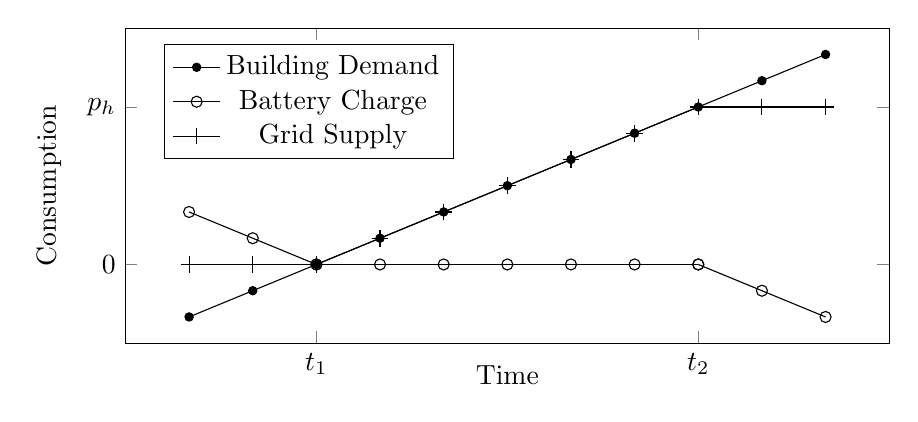
\begin{tikzpicture}

\begin{axis}[
width=0.8\columnwidth,height=4cm,scale only axis,
axis line style={-}, xtick style={-}, ytick style={-},
xlabel=Time,
ylabel=Consumption,
every axis y label/.style={at={(-0.1,0.5)},rotate=90,anchor=center}, 
every axis x label/.style={at={(0.5,-0.1)},anchor=center}, 
%grid=both, grid style={style=densely dotted},
xtick={2,8},
xticklabels={$t_1$,$t_2$},
ytick={0,6},
yticklabels={$0$,$p_h$},
legend style={at={(0.05,0.95)},anchor=north west}
] 

% Draw the Demand-Supply curve
\addplot[-,mark=*,mark size=1.5] expression[domain=0:10,samples=11] {x-2};
\addlegendentry{Building Demand} 

% Draw the Battery curve
\addplot[-,mark=o,mark size=2] expression[forget plot,domain=0:2,samples=3] {2-x}; 
\addplot[-,mark=o,mark size=2] expression[forget plot,domain=2:8,samples=7] {0}; 
\addplot[-,mark=o,mark size=2] expression[domain=8:10,samples=3] {8-x}; 
\addlegendentry{Battery Charge} 

% Draw the Grid supply curve
\addplot[-,mark=+,mark size=3] expression[forget plot,domain=0:2,samples=3] {0}; 
\addplot[-,mark=+,mark size=3] expression[forget plot,domain=2:8,samples=7] {x-2}; 
\addplot[-,mark=+,mark size=3] expression[domain=8:10,samples=3] {6}; 
\addlegendentry{Grid Supply} 
\end{axis} 
\end{tikzpicture} 

%}
}
\qquad
\subfigure[Goal-plan hierarchy for a $k$-modules battery system.]{\label{fig:gptree}
%\resizebox{0.9\columnwidth}{!}{
%!TEX root = ../aamas11storage.tex
\begin{tikzpicture} [level distance=8.0em]
\tikzstyle{planbox}=[draw,text width=11.0em,rectangle split,rectangle split parts=3]
\tikzstyle{goalbox}=[draw,rounded corners=1.25em,minimum height=3em,minimum width=5em]

	
\tikzstyle{level 1}=[sibling distance=13.0em] 
\tikzstyle{level 2}=[level distance=7.0em] 

\node[goalbox,solid] {$G($r,k,s$)$}
	child {node[planbox] {$SetCharge$ 
			\nodepart{second} $\psi:satisfies(r,k,s,C),$\\$k>0$
			\nodepart{third} $set(k,C)$
		}
		child {node[goalbox] {$G($r,k-1,s'$)$}}
	}
	child {node[planbox] {$SetDischarge$ \nodepart{second}
			\nodepart{second} $\psi:satisfies(r,k,s,D),$\\$k>0$
			\nodepart{third} $set(k,D)$
		}
		child {node[goalbox] {$G($r,k-1,s'$)$}}
	}
	child {node[planbox] {$SetNotUsed$ \nodepart{second}
			\nodepart{second} $\psi:satisfies(r,k,s,N),$\\$k>0$
			\nodepart{third} $set(k,N)$
		}
		child {node[goalbox] {$G($r,k-1,s'$)$}}
	}
	child {node[planbox] {$Execute$ 
			\nodepart{second} $\psi:k==0$
			\nodepart{third} $operate()$ \\$evaluate()$
		}
	}
;

\end{tikzpicture}



%}
}
\caption{An energy storage application.}
\end{center}
\label{fig:energystorage}
\end{figure*}


%\notemin{SS: I am here}
%The energy storage domain scenario (c.f. Section \ref{sec:application}) highlights the benefits of our dynamic confidence measure of Equation \ref{eqn:confidence}. In this domain it is easy to think of situations where the dynamics of the environment changes such that the solution space varies over time. For instance, our motivation for learning is that battery chemistry (and therefore performance) deteriorates over time, and the system should learn to avoid solutions that no longer work in the future. However, worn battery modules get replaced every now and then, and hence, some configurations that the learner may have eliminated previously may become applicable once again. Similar examples may be developed for situations involving module malfunctions. The point is that each such change in the environment impacts the solution space in some way, however an explicit notification, that may be used to trigger a change in behaviour, is not always available (some changes may be continuous, for instance). Moreover, several such factors may play on the solution space at one time, and it is up to the learner to respond in this environment appropriately.


%Here it becomes important for an agent to reliably recognise such changes, and respond by adjusting its exploration strategy accordingly (or perhaps, switching policies, choosing to learn afresh, and so on). Since the new confidence measure is built using observed data alone, it consequently reflects agent performance: our confidence is maximum when the rate of change in observed performance and worlds states is stable, and minimum when it is not. Importantly, this means that the measure is non-monotonic and as such may be used to dynamically tune the exploration strategy (for instance during plan selection as in Equation \ref{eqn:omega}) against a variable solution space.
